\documentclass[a4paper, 12pt]{article}

% --- PACOTES ---
% --- Codificação e Fontes ---
\usepackage[utf8]{inputenc}
\usepackage[T1]{fontenc}
\usepackage{lmodern}
\usepackage[brazil]{babel}
\usepackage{microtype}

% --- Layout e Estrutura ---
\usepackage{geometry}
\usepackage{graphicx}
\usepackage{float}

% --- Tabelas ---
\usepackage{array}
\usepackage{longtable}
\usepackage{booktabs}
\usepackage{ragged2e}

% --- Citações e Referências ---
\usepackage{natbib}

% --- Listas ---
\usepackage{enumitem}
\newlist{compactitem}{itemize}{1}
\setlist[compactitem]{label=\textbullet, topsep=0pt, partopsep=0pt, itemsep=0pt, parsep=0pt, leftmargin=*}

% --- Links ---
\usepackage[hidelinks]{hyperref}

\geometry{
    a4paper,
    left=2.5cm,
    right=2.5cm,
    top=2.5cm,
    bottom=2.5cm,
}

\graphicspath{{figures/}}

\begin{document}

% --- PÁGINA DE ROSTO ---
\begin{titlepage}
    \centering
    
\includegraphics[width=0.4\textwidth]{upe.png}\par
    \vspace{1.5cm}

    {\large UNIVERSIDADE DE PERNAMBUCO - UPE}\par
    \vspace{0.2cm}
    {\large ESCOLA POLITÉCNICA DE PERNAMBUCO - POLI}

    \vfill

    {\Large \textbf{RELATÓRIO DE ANÁLISE EXPLORATÓRIA}}\par

    \vspace{1cm}

    {\huge \bfseries ANOMALY DETECTION IN C2 BEACONING TRAFFIC USING PRIVACY-PRESERVING FEDERATED LEARNING\\CTU-13 DATASET EDA}\par

    \vfill

    \begin{flushleft}
    \large
        \textbf{Alunos:} Gabriel Souza Borges, Ranie Campos Lins \\
        \textbf{Orientador:} Prof. Dr. Bruno José Torres Fernandes \\
        \textbf{Co-Orientador:} Prof. Dr. Leandro Honorato de Souza Silva
    \end{flushleft}

    \vfill

    \large
    Recife-PE \\
    \today
\end{titlepage}

\tableofcontents
\listoffigures
\listoftables

\newpage

\section{Introdução}
O presente relatório documenta a análise exploratória do conjunto de dados CTU-13, etapa essencial do cronograma do trabalho ``Anomaly Detection in C2 Beaconing Traffic Using Privacy-Preserving Federated Learning''. O objetivo é compreender o comportamento do tráfego rotulado como botnet, normal e background, bem como avaliar a cobertura de cenários disponível para experimentos de aprendizado federado focados em detecção de beaconing.

\section{Metodologia}
A análise foi desenvolvida no notebook \texttt{notebooks/eda\_ctu13.ipynb}, considerando o export NetFlow bidirecional recomendado pelos mantenedores do CTU-13. As principais etapas foram:
\begin{compactitem}
    \item Conversão de carimbos de tempo para \texttt{datetime} e normalização de portas representadas em hexadecimal.
    \item Cast de colunas categóricas (\texttt{Proto}, \texttt{Dir}, \texttt{State}, \texttt{Label}) para \texttt{category}, reduzindo o uso de memória para aproximadamente 1{,}9~GB.
    \item Criação do indicador binário \texttt{is\_botnet} para separar fluxos maliciosos do tráfego de fundo.
    \item Geração de figuras e tabelas exportadas para \texttt{docs/figures} e \texttt{docs/tables}, permitindo reprodução direta neste relatório.
\end{compactitem}

\section{Visão Geral do Dataset}
O CTU-13 é composto por treze cenários capturados em 2011 na Universidade Tcheca de Tecnologia (CTU), disponibilizados pelo Stratosphere Laboratory\footnote{Sebastian Garcia, Martin Grill, Jan Stiborek e Alejandro Zunino. ``An empirical comparison of botnet detection methods''. \textit{Computers \& Security}, 45:100--123, 2014.}. Cada cenário combina tráfego de botnets com atividades legítimas e de background. A amostra processada contém mais de 2,8 milhões de fluxos, dos quais 40~961 são rotulados como botnet.

Os principais rótulos encontrados estão listados na Tabela\,\ref{tab:label_summary}. Observa-se predominância de fluxos de background, enquanto o cenário V42 concentra a maior parte dos eventos maliciosos disponíveis, fornecendo um ponto de partida claro para experimentos de detecção.

\begin{longtable}{lrrrrrr}
\caption{Top 20 Labels by Flow Count} \label{tab:label_summary} \\
\toprule
Label & Flows & Flow_Percentage & Avg_Duration_s & Avg_Total_Packets & Avg_Total_Bytes & Avg_Source_Bytes \\
\midrule
\endfirsthead
\caption[]{Top 20 Labels by Flow Count} \\
\toprule
Label & Flows & Flow_Percentage & Avg_Duration_s & Avg_Total_Packets & Avg_Total_Bytes & Avg_Source_Bytes \\
\midrule
\endhead
\midrule
\multicolumn{7}{r}{Continued on next page} \\
\midrule
\endfoot
\bottomrule
\endlastfoot
flow=Background-UDP-Established & 1169677 & 41.41 & 928.15 & 6.14 & 1682.45 & 441.45 \\
flow=To-Background-UDP-CVUT-DNS-Server & 941706 & 33.34 & 0.71 & 2.00 & 244.08 & 80.39 \\
flow=Background-TCP-Established & 223543 & 7.91 & 90.05 & 139.66 & 116200.85 & 35628.81 \\
flow=Background-Established-cmpgw-CVUT & 137257 & 4.86 & 232.33 & 138.78 & 134791.94 & 8908.24 \\
flow=Background-TCP-Attempt & 105438 & 3.73 & 29.65 & 2.81 & 184.85 & 130.29 \\
flow=Background-UDP-Attempt & 66699 & 2.36 & 584.41 & 8.18 & 1136.67 & 1136.01 \\
flow=Background & 40216 & 1.42 & 662.80 & 91.54 & 35675.78 & 28135.56 \\
flow=Background-Attempt-cmpgw-CVUT & 30983 & 1.10 & 137.14 & 2.61 & 292.51 & 292.49 \\
flow=From-Botnet-V42-UDP-DNS & 26140 & 0.93 & 1.10 & 2.00 & 257.86 & 73.38 \\
flow=To-Background-CVUT-Proxy & 19542 & 0.69 & 49.26 & 277.83 & 223645.58 & 14618.57 \\
flow=From-Normal-V42-Stribrek & 18438 & 0.65 & 22.57 & 16.74 & 11749.52 & 1974.36 \\
flow=From-Botnet-V42-TCP-Attempt-SPAM & 8105 & 0.29 & 28.09 & 3.13 & 194.27 & 194.27 \\
flow=From-Normal-V42-Grill & 7654 & 0.27 & 42.92 & 71.36 & 68044.38 & 2423.06 \\
flow=From-Normal-V42-Jist & 3808 & 0.13 & 41.78 & 14.54 & 7690.79 & 816.20 \\
flow=From-Botnet-V42-UDP-Attempt-DNS & 3057 & 0.11 & 0.01 & 1.00 & 72.47 & 72.47 \\
flow=To-Background-CVUT-WebServer & 2587 & 0.09 & 22.69 & 110.17 & 98549.09 & 3122.93 \\
flow=Background-UDP-NTP-Established-1 & 2233 & 0.08 & 2275.35 & 22.43 & 2018.49 & 1009.87 \\
flow=From-Botnet-V42-TCP-Attempt & 1881 & 0.07 & 31.93 & 3.13 & 199.86 & 174.62 \\
flow=Background-ajax.google & 1197 & 0.04 & 62.04 & 19.44 & 6523.69 & 2196.05 \\
flow=To-Background-MatLab-Server & 833 & 0.03 & 30.79 & 2.92 & 205.62 & 45.36 \\
\end{longtable}


\section{Análise Exploratória dos Fluxos}
\subsection{Distribuição de Rótulos}
A Figura\,\ref{fig:label_distribution} sintetiza a distribuição dos rótulos (topo \emph{Top 10 + Others}). O tráfego de background domina o conjunto, destacando a necessidade de técnicas de detecção de anomalias capazes de lidar com forte desbalanceamento.

\begin{figure}[H]
    \centering
    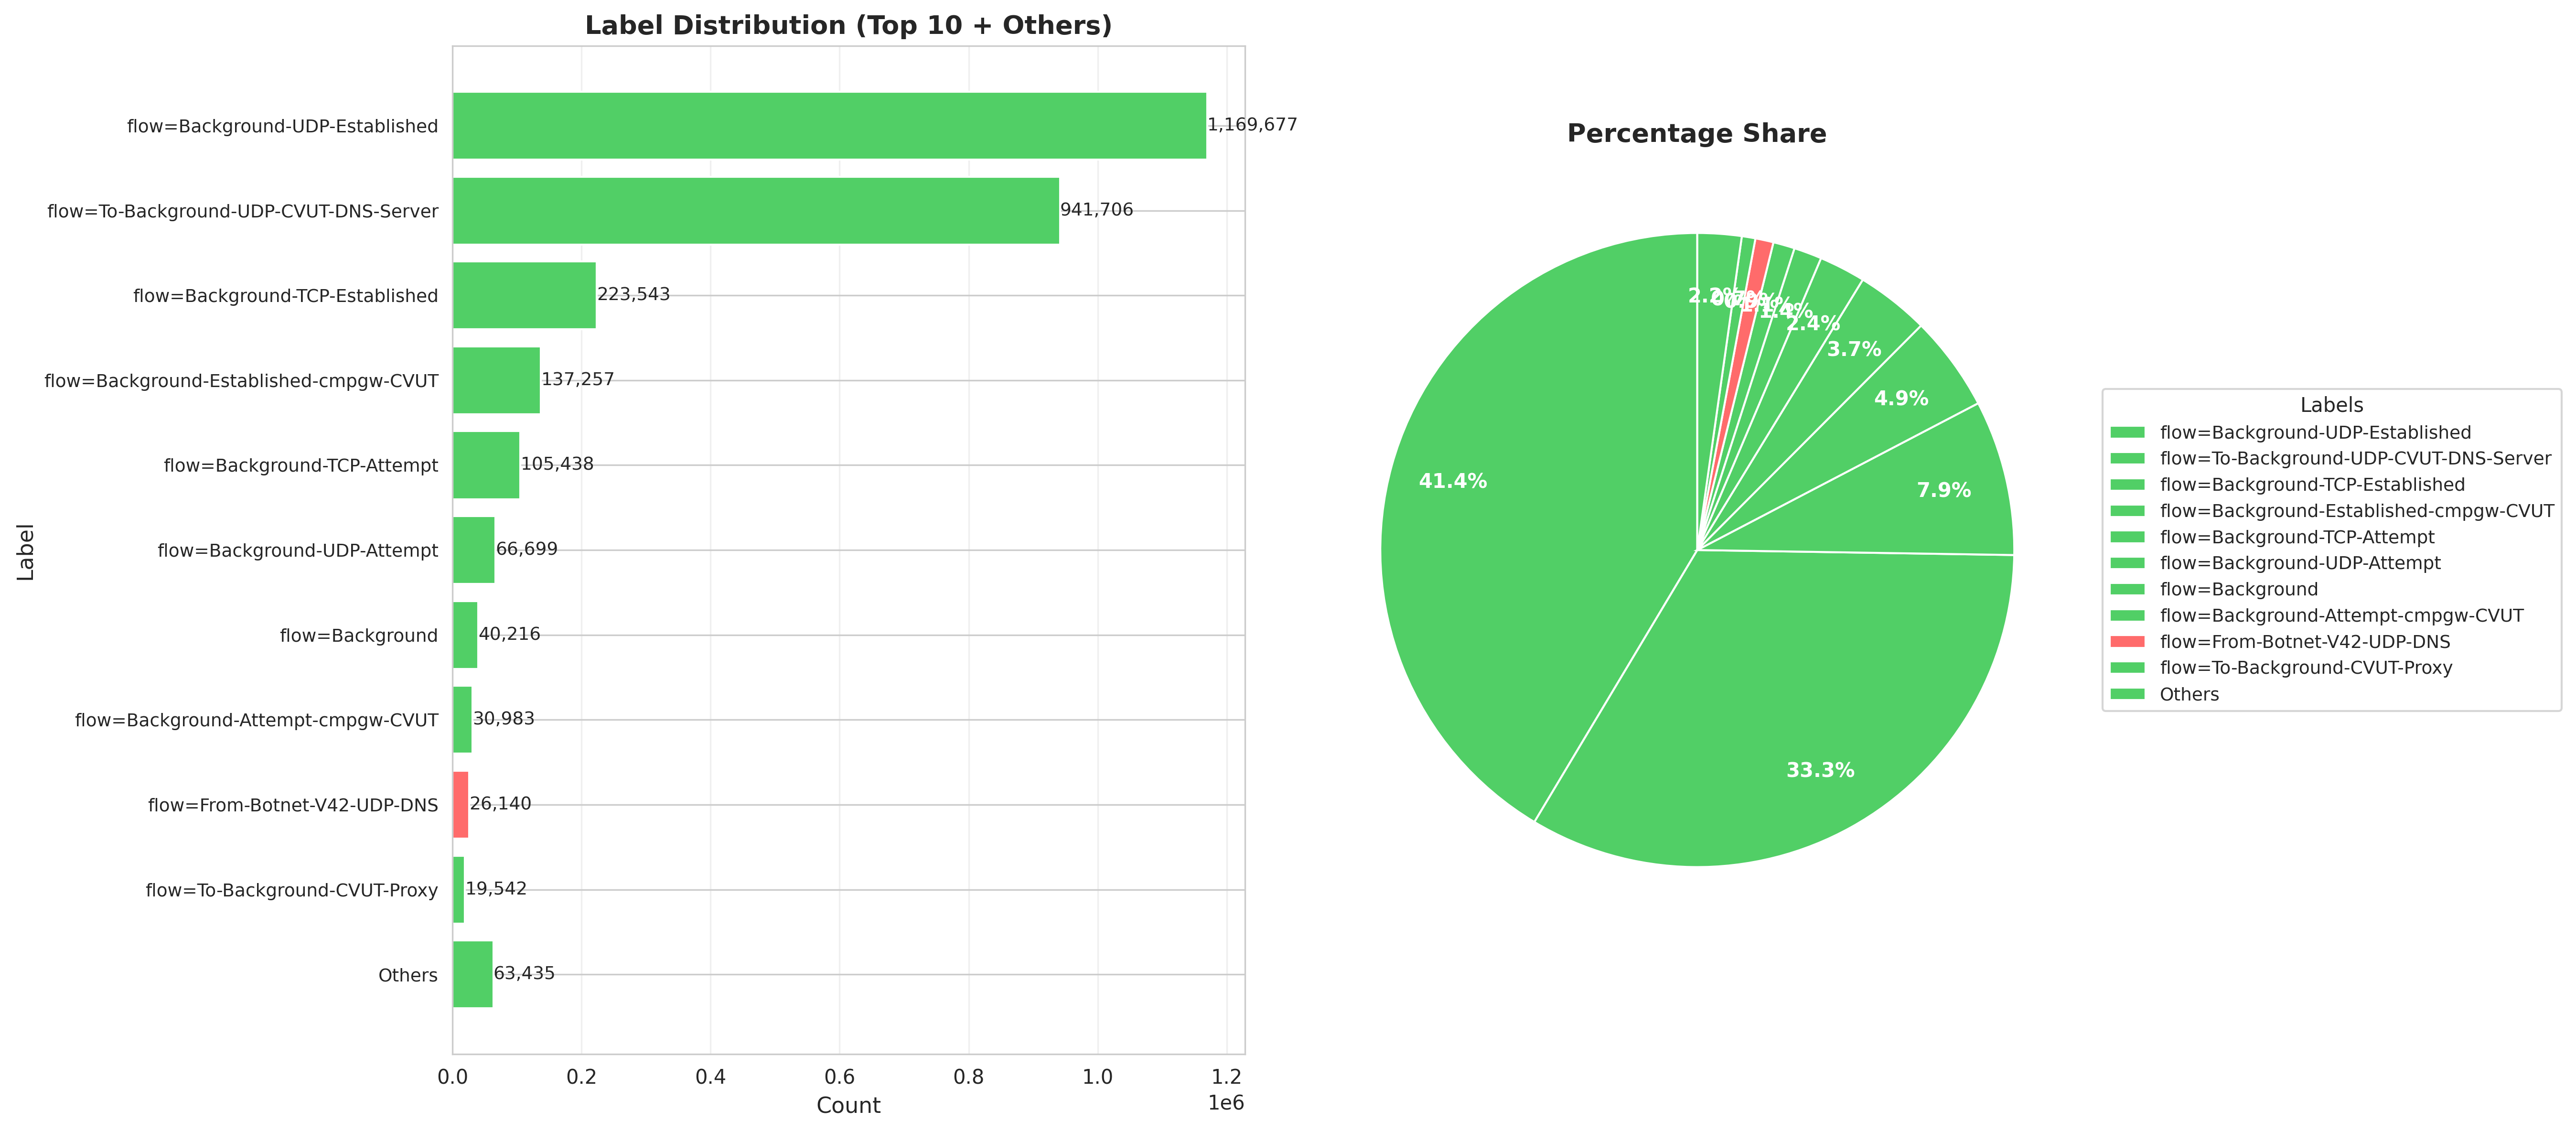
\includegraphics[width=0.9\textwidth]{label_distribution.png}
    \caption{Distribuição dos rótulos no subconjunto CTU-13 analisado.}
    \label{fig:label_distribution}
\end{figure}

\subsection{Estados de Conexão}
A Figura\,\ref{fig:connection_state} apresenta o histograma de estados de conexão em escala logarítmica. Identificam-se 230 estados distintos, reforçando a diversidade comportamental presente no tráfego e a importância de atributos de estado na modelagem de beaconing.

\begin{figure}[H]
    \centering
    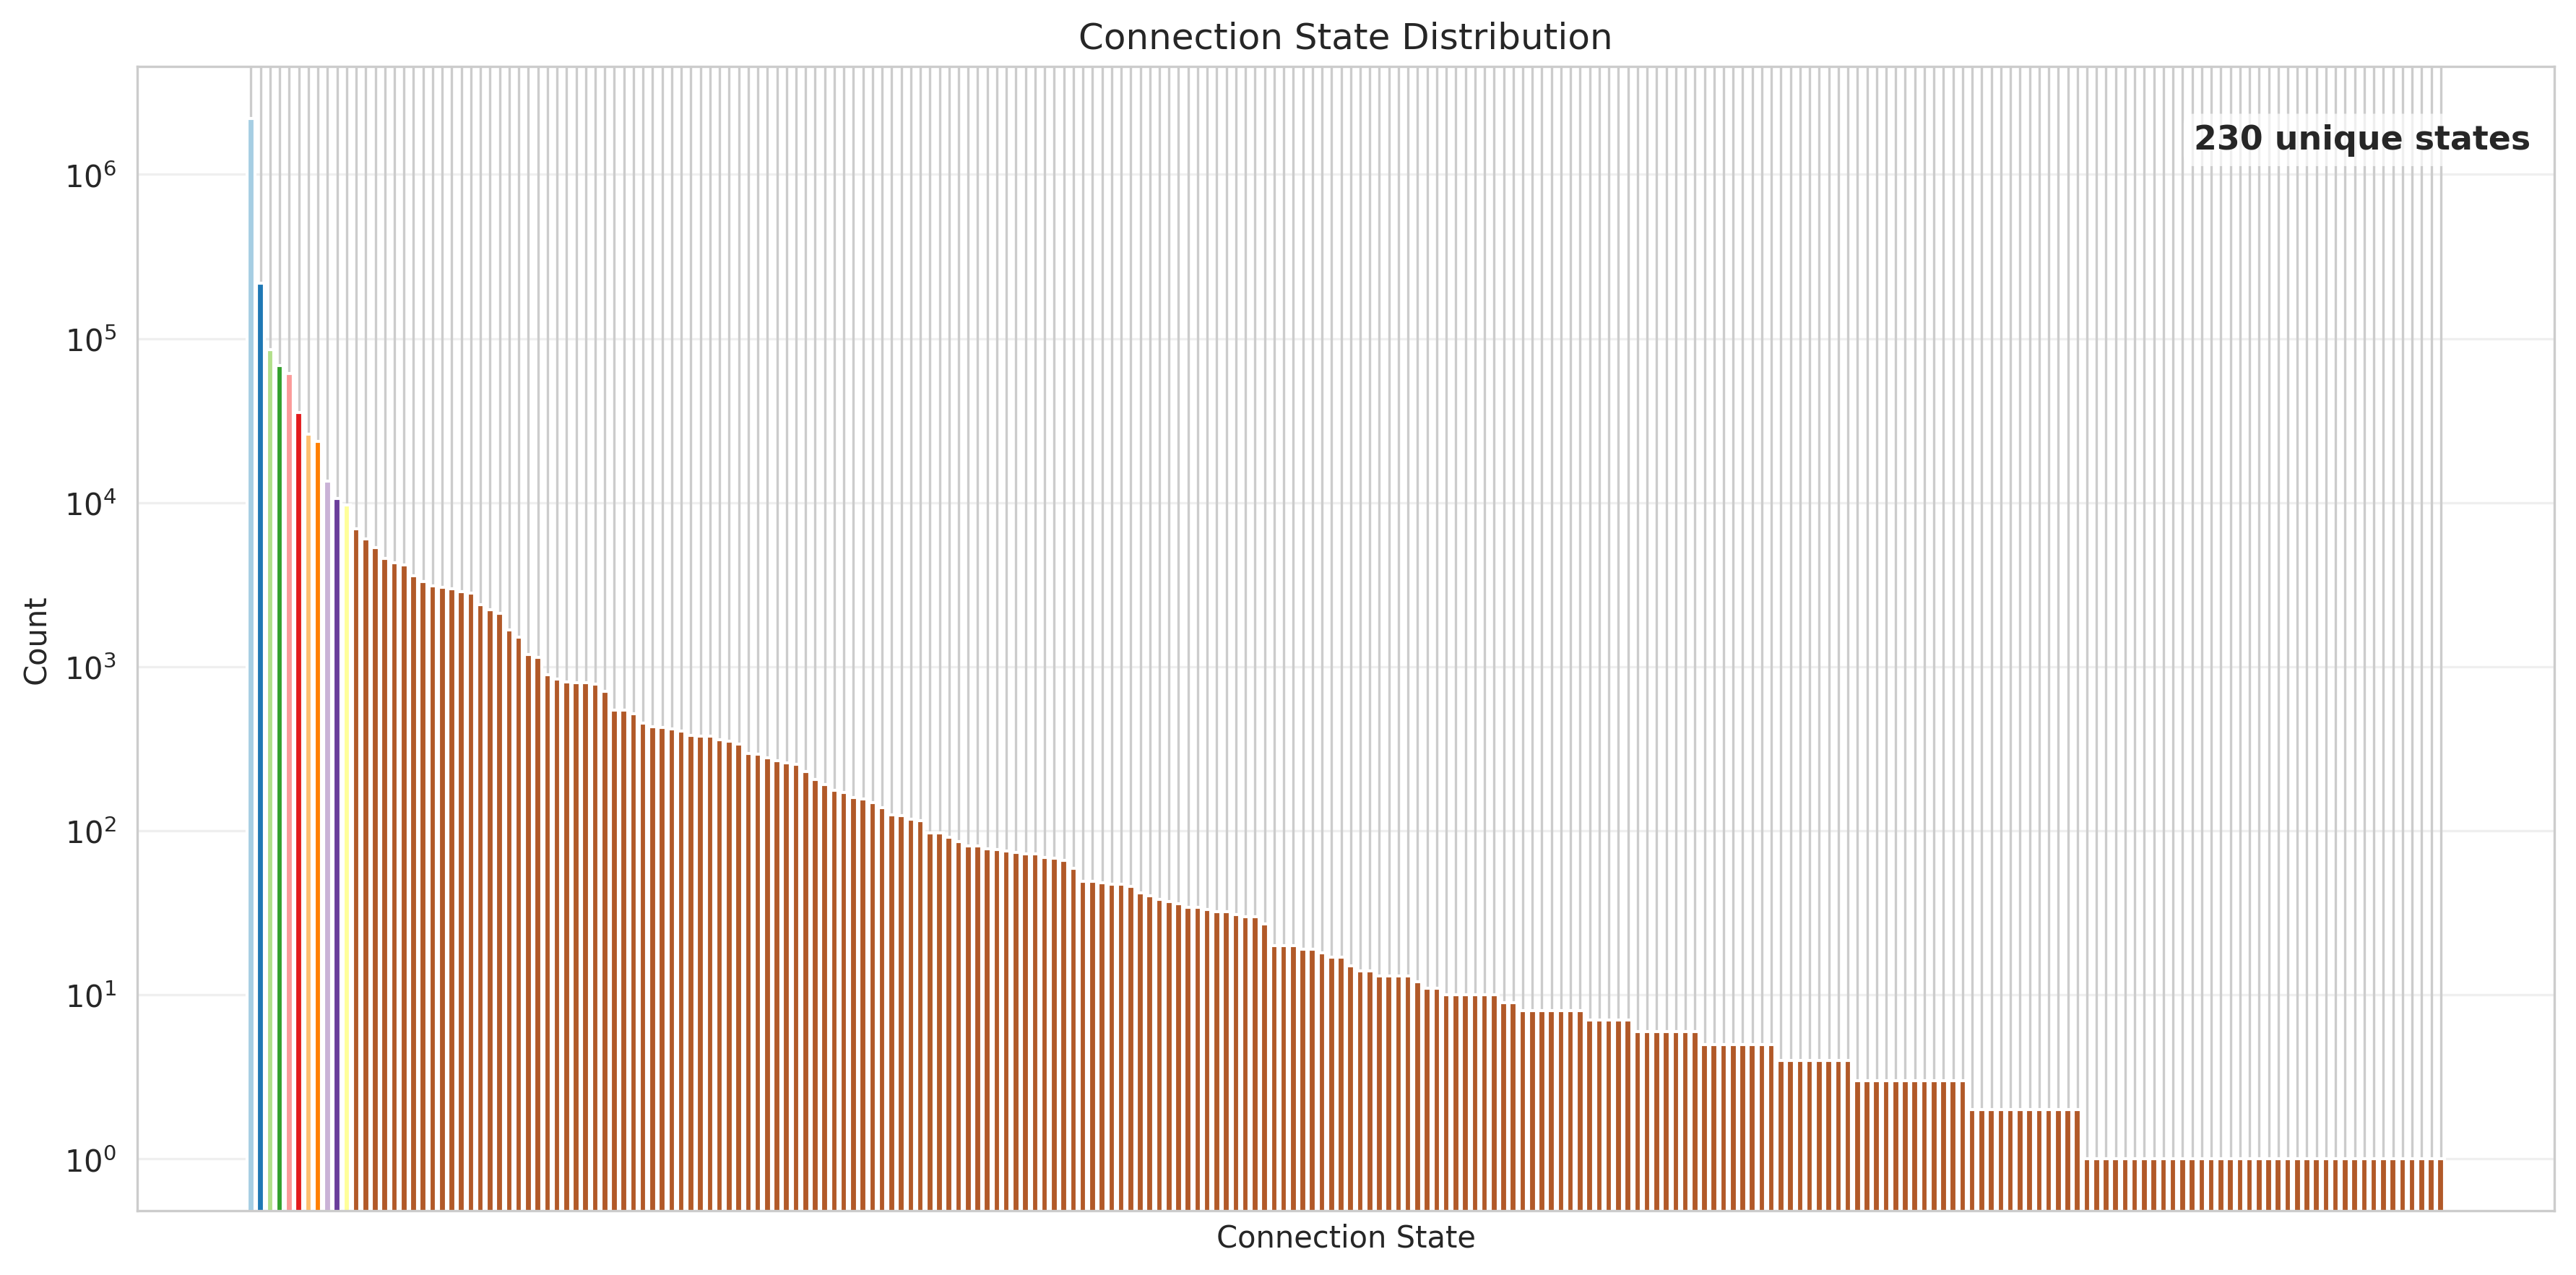
\includegraphics[width=0.85\textwidth]{connection_state_distribution.png}
    \caption{Distribuição dos estados de conexão (escala log).}
    \label{fig:connection_state}
\end{figure}

\subsection{Comparação Botnet vs Background}
A Figura\,\ref{fig:botnet_background} compara botnet e background quanto a duração, total de pacotes, total de bytes e protocolos utilizados. Fluxos maliciosos exibem durações e volumes significativamente menores, enquanto UDP e TCP aparecem como protocolos dominantes em ambos os grupos, com proporções distintas. Esses contrastes reforçam a hipótese de tráfego beaconing com janelas de comunicação curtas e regulares.

\begin{figure}[H]
    \centering
    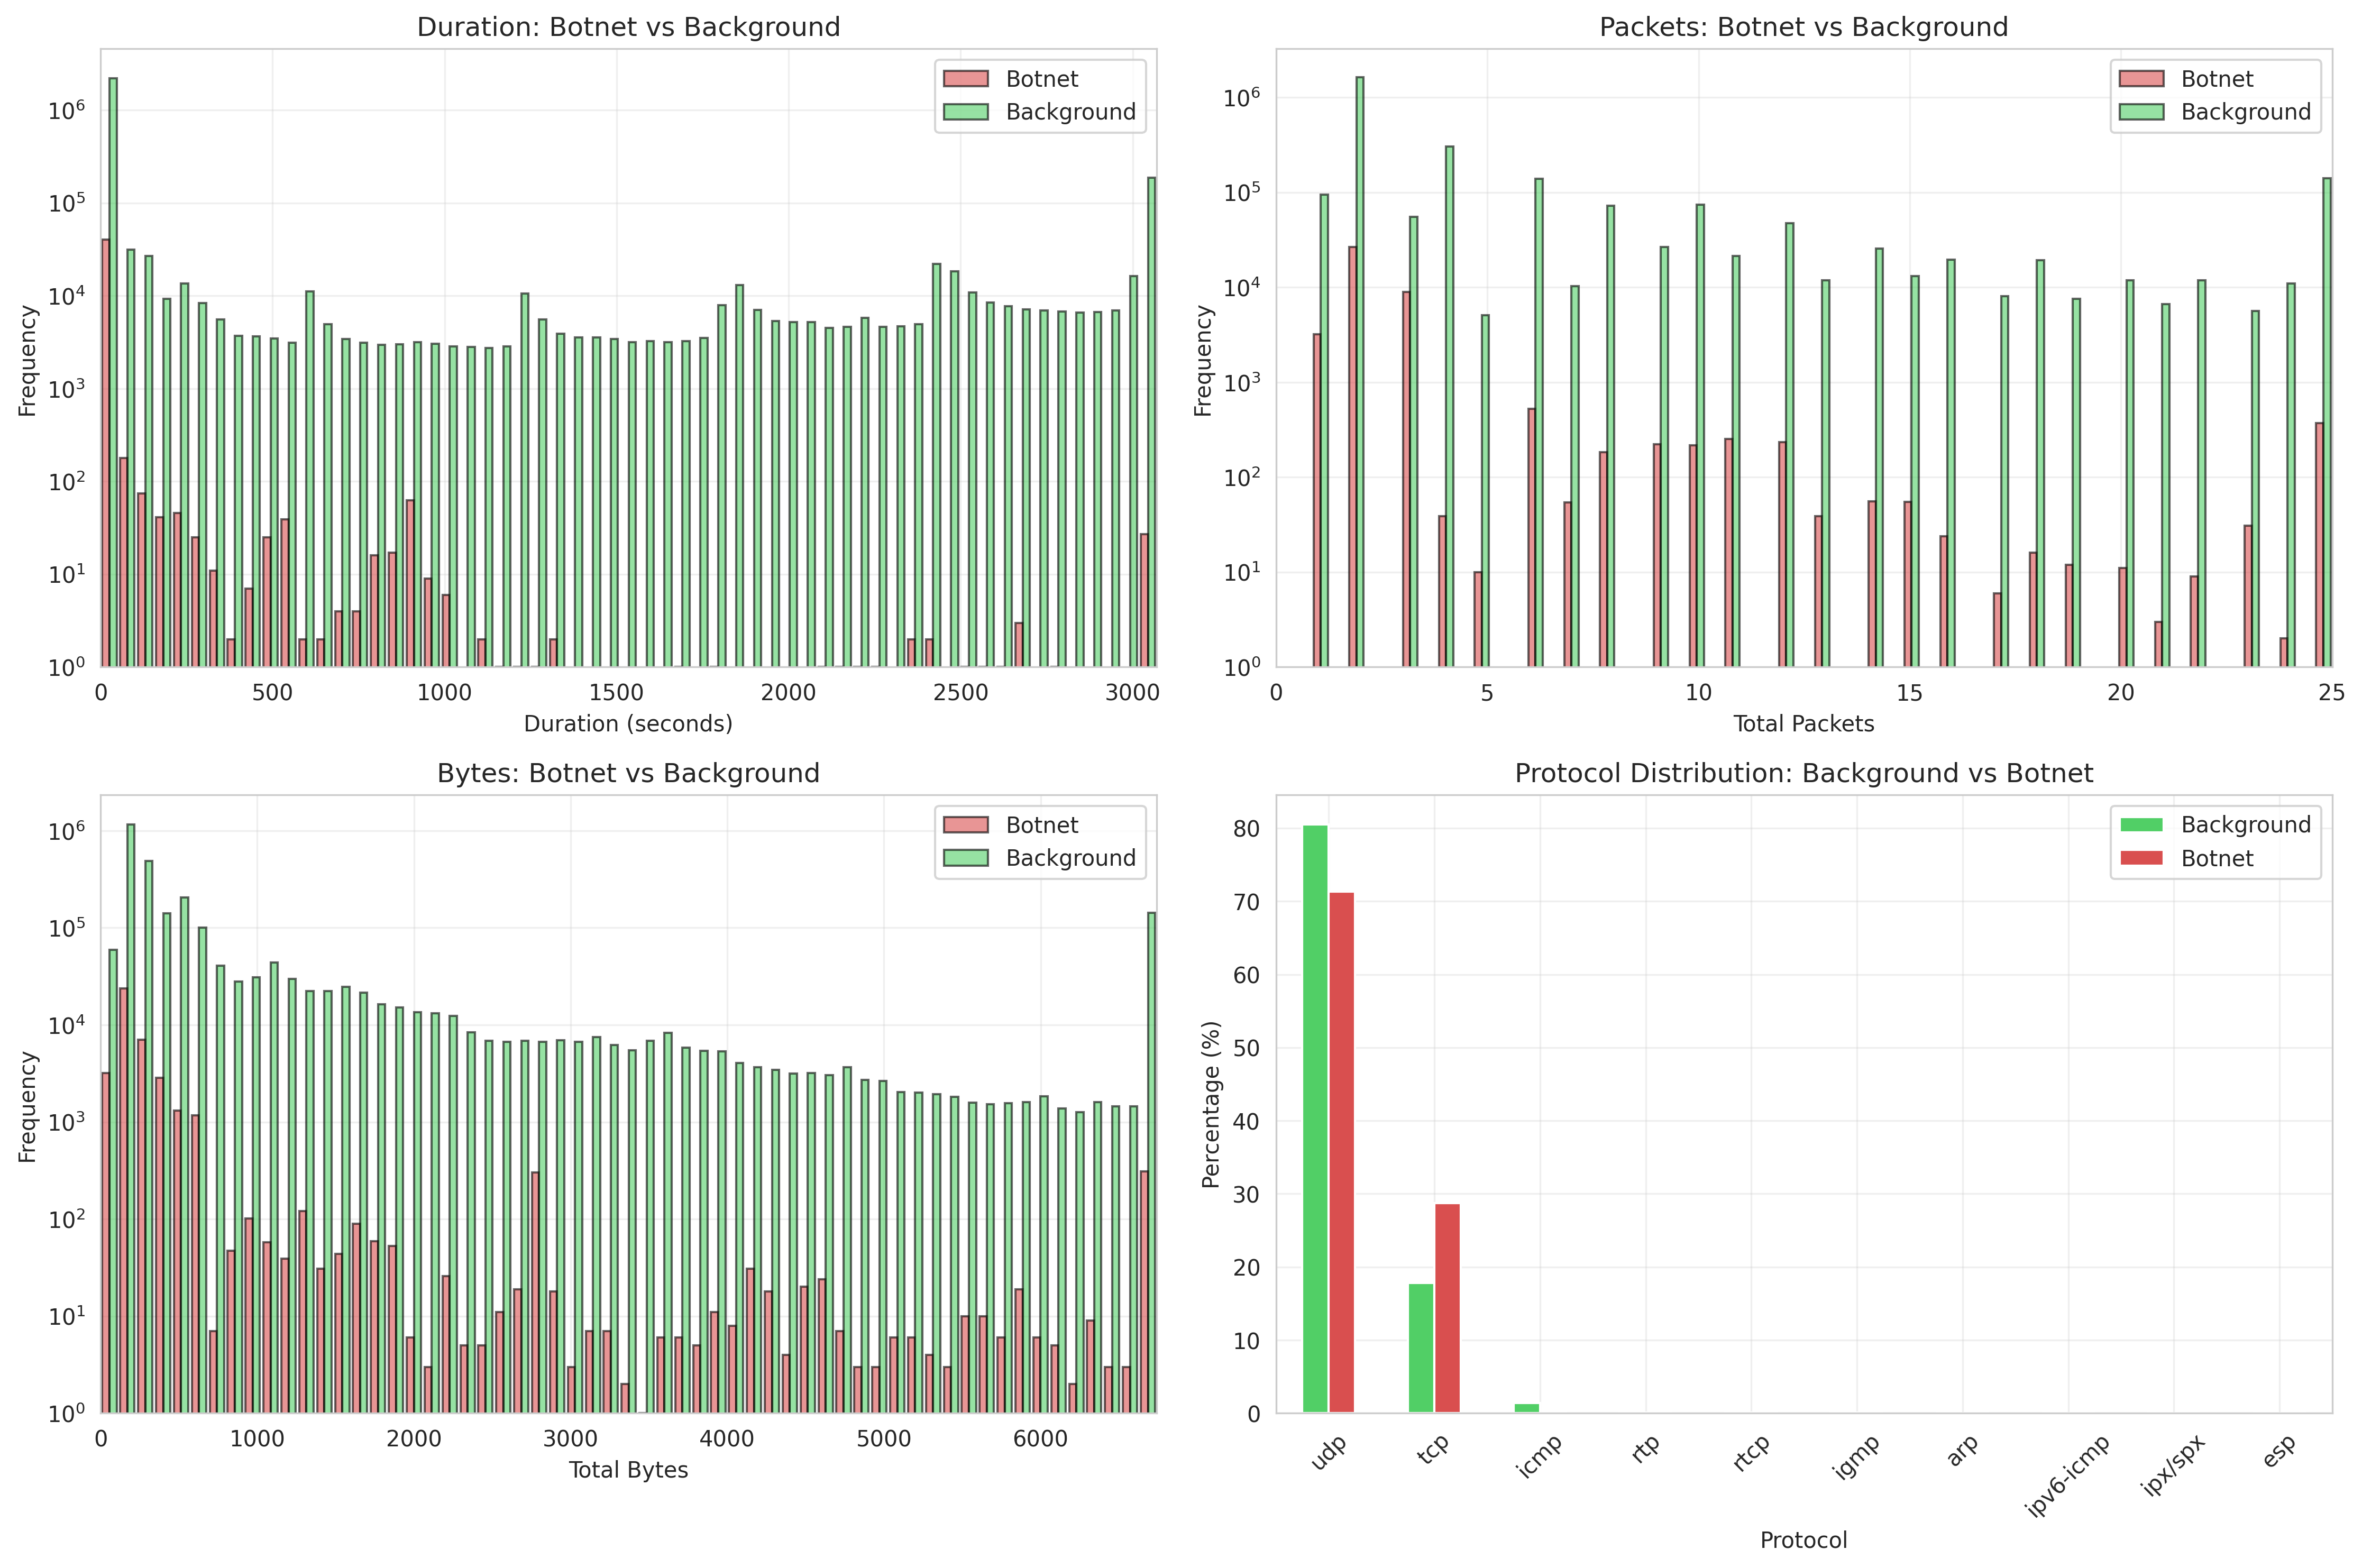
\includegraphics[width=0.9\textwidth]{botnet_vs_background.png}
    \caption{Distribuição de duração, pacotes, bytes e protocolos para botnet e background.}
    \label{fig:botnet_background}
\end{figure}

\section{Cobertura de Cenários}
A Tabela\,\ref{tab:scenario_counts} mostra a cobertura de cenários inferida a partir dos rótulos. O cenário V42 é o único com anotações explícitas de botnet neste subconjunto, enquanto o restante dos fluxos se mantém sem identificação de cenário, servindo como tráfego ambiente.

\begin{table}
\caption{Scenario Coverage in CTU-13 Subset}
\label{tab:scenario_counts}
\begin{tabular}{lrr}
\toprule
Scenario & Flows & Percentage \\
\midrule
Unknown & 2753288 & 97.47 \\
V42 & 71348 & 2.53 \\
\bottomrule
\end{tabular}
\end{table}


A Tabela\,\ref{tab:scenario_label_mix} detalha a proporção de fluxos botnet e background por cenário. Aproximadamente 57\% dos fluxos em V42 são rotulados como botnet, oferecendo uma base rica para avaliação de técnicas de detecção de beaconing sob forte desbalanceamento.

\begin{table}
\caption{Label Mix by Scenario}
\label{tab:scenario_label_mix}
\begin{tabular}{lrrrrr}
\toprule
Scenario & Background\_Normal & Botnet & Total & Botnet\_pct & Background\_pct \\
\midrule
Unknown & 2753288 & 0 & 2753288 & 0.00 & 100.00 \\
V42 & 30387 & 40961 & 71348 & 57.41 & 42.59 \\
\bottomrule
\end{tabular}
\end{table}


\section{Implicações para Aprendizado Federado}
Com base nos resultados anteriores (Figuras\,\ref{fig:label_distribution} e \ref{fig:botnet_background} e Tabelas\,\ref{tab:scenario_counts} e \ref{tab:scenario_label_mix}), propõe-se utilizar o cenário V42 como nodo ``infectado'' em um ambiente federado, enquanto o grande conjunto de fluxos de background pode ser particionado entre clientes adicionais para simular organizações distintas. Essa configuração favorece experimentos de detecção de anomalias preservando privacidade, pois os dados crus permanecem localizados em cada cliente. As diferenças em duração e volume de tráfego entre botnet e background apontam para atributos promissores em modelos baseados em séries temporais ou estatísticas agregadas.

\section{Próximos Passos}
Os próximos passos previstos incluem:
\begin{compactitem}
    \item Incorporar cenários adicionais do CTU-13 para ampliar a diversidade de botnets analisadas.
    \item Definir estratégia de amostragem e normalização para treinamento federado.
    \item Projetar métricas de beaconing (intervalos, periodicidade, entropia de portas) a partir dos NetFlows.
    \item Integrar as descobertas em pipelines de aprendizado federado com mecanismos de preservação de privacidade.
\end{compactitem}

\section{Conclusão}
A análise exploratória evidencia forte desbalanceamento entre tráfego benigno e malicioso, além de padrões específicos de fluxos botnet compatíveis com comunicação C2 em modo beaconing. Esses achados orientam tanto a seleção de atributos quanto a arquitetura de experimentos federados, estabelecendo uma base quantitativa para as etapas subsequentes do projeto.

\end{document}
